\documentclass[12pt, oneside]{article} % Default font size and left-justified equations
\usepackage[top=1.5cm,bottom=3cm,left=3.2cm,right=3.2cm,headsep=10pt]{geometry} % Page margins
\usepackage{xcolor} % Required for specifying colors by name
\definecolor{ocre}{RGB}{243,102,25} % Define the orange color used for highlighting throughout the book
\usepackage{avant} % Use the Avantgarde font for headings
\usepackage{mathptmx} % Use the Adobe Times Roman as the default text font together with math symbols from the Sym­bol, Chancery and 
\usepackage{color}
\usepackage{microtype} % Slightly tweak font spacing for aesthetics
\usepackage[utf8]{inputenc} % Required for including letters with accents
\usepackage[T1]{fontenc} % Use 8-bit encoding that has 256 glyphs
\usepackage{titlesec} % Allows customization of titles
\usepackage{graphicx} % Required for including pictures
\graphicspath{{Pictures/}} % Specifies the directory where pictures are stored
\usepackage{tikz} % Required for drawing custom shapes
\usepackage[spanish]{babel} % English language/hyphenation
\usepackage{enumitem} % Customize lists
\setlist{nolistsep} % Reduce spacing between bullet points and numbered lists
\usepackage{booktabs} % Required for nicer horizontal rules in tables
\usepackage{eso-pic}
\usepackage{url}
\usepackage{helvet}
\renewcommand{\familydefault}{\sfdefault}
\usepackage{fancyhdr}
\pagestyle{fancy}

%--------color de portada-----------------
\definecolor{titlepagecolor}{cmyk}{1,.60,0,.40}
\definecolor{namecolor}{cmyk}{0,0,0,0}
\definecolor{titlecolor}{RGB}{255,127,36}
\definecolor{liccolor}{RGB}{32,178,170}
%--------color de portada-----------------

\setlength{\parindent}{2cm}
\setlength{\parskip}{\baselineskip} 

\renewcommand{\baselinestretch}{1.2}

\begin{document}

%----------------------------------------------------------------------------------------
%    TITLE PAGE
%----------------------------------------------------------------------------------------
%2 page
%%%%%%%%%%%%%%%%
\begin{titlepage}


\normalsize
\vspace*{12cm} 

\noindent

 \begin{minipage}{\textwidth}
  \parbox[t]{1.2\linewidth}{
 \begin{flushright}
            \centering
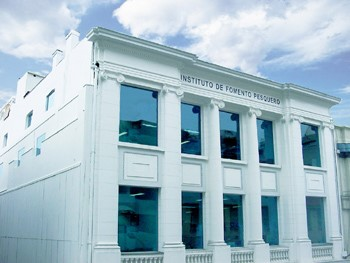
\includegraphics[height=5.2cm]{Figuras/Portada1_Final.jpg} \\
 ----------------------------------------------------\\
 \fontsize{11pt}{10pt}\selectfont 	
 \textbf{INSTITUTO DE FOMENTO PESQUERO} \\
 Almte. Manuel Blanco Encalada 839 \\ 
 Fono 56-32-2151500 \\
 Valparaíso, Chile \\
\textbf{www.ifop.cl} \\
 ----------------------------------------------------\\
\end{flushright} 
}
 \end{minipage}


\vfill
\end{titlepage}

%%%%%%%%%%%%%%%%%%
% PAGINA 2
%%%%%%%%%%%%%%%%%%

\begingroup
\begin{titlepage}
    \newgeometry{left=2.5cm,top=0cm,bottom=1cm, right=2.5cm}
    \AddToShipoutPicture*{\put(0,0){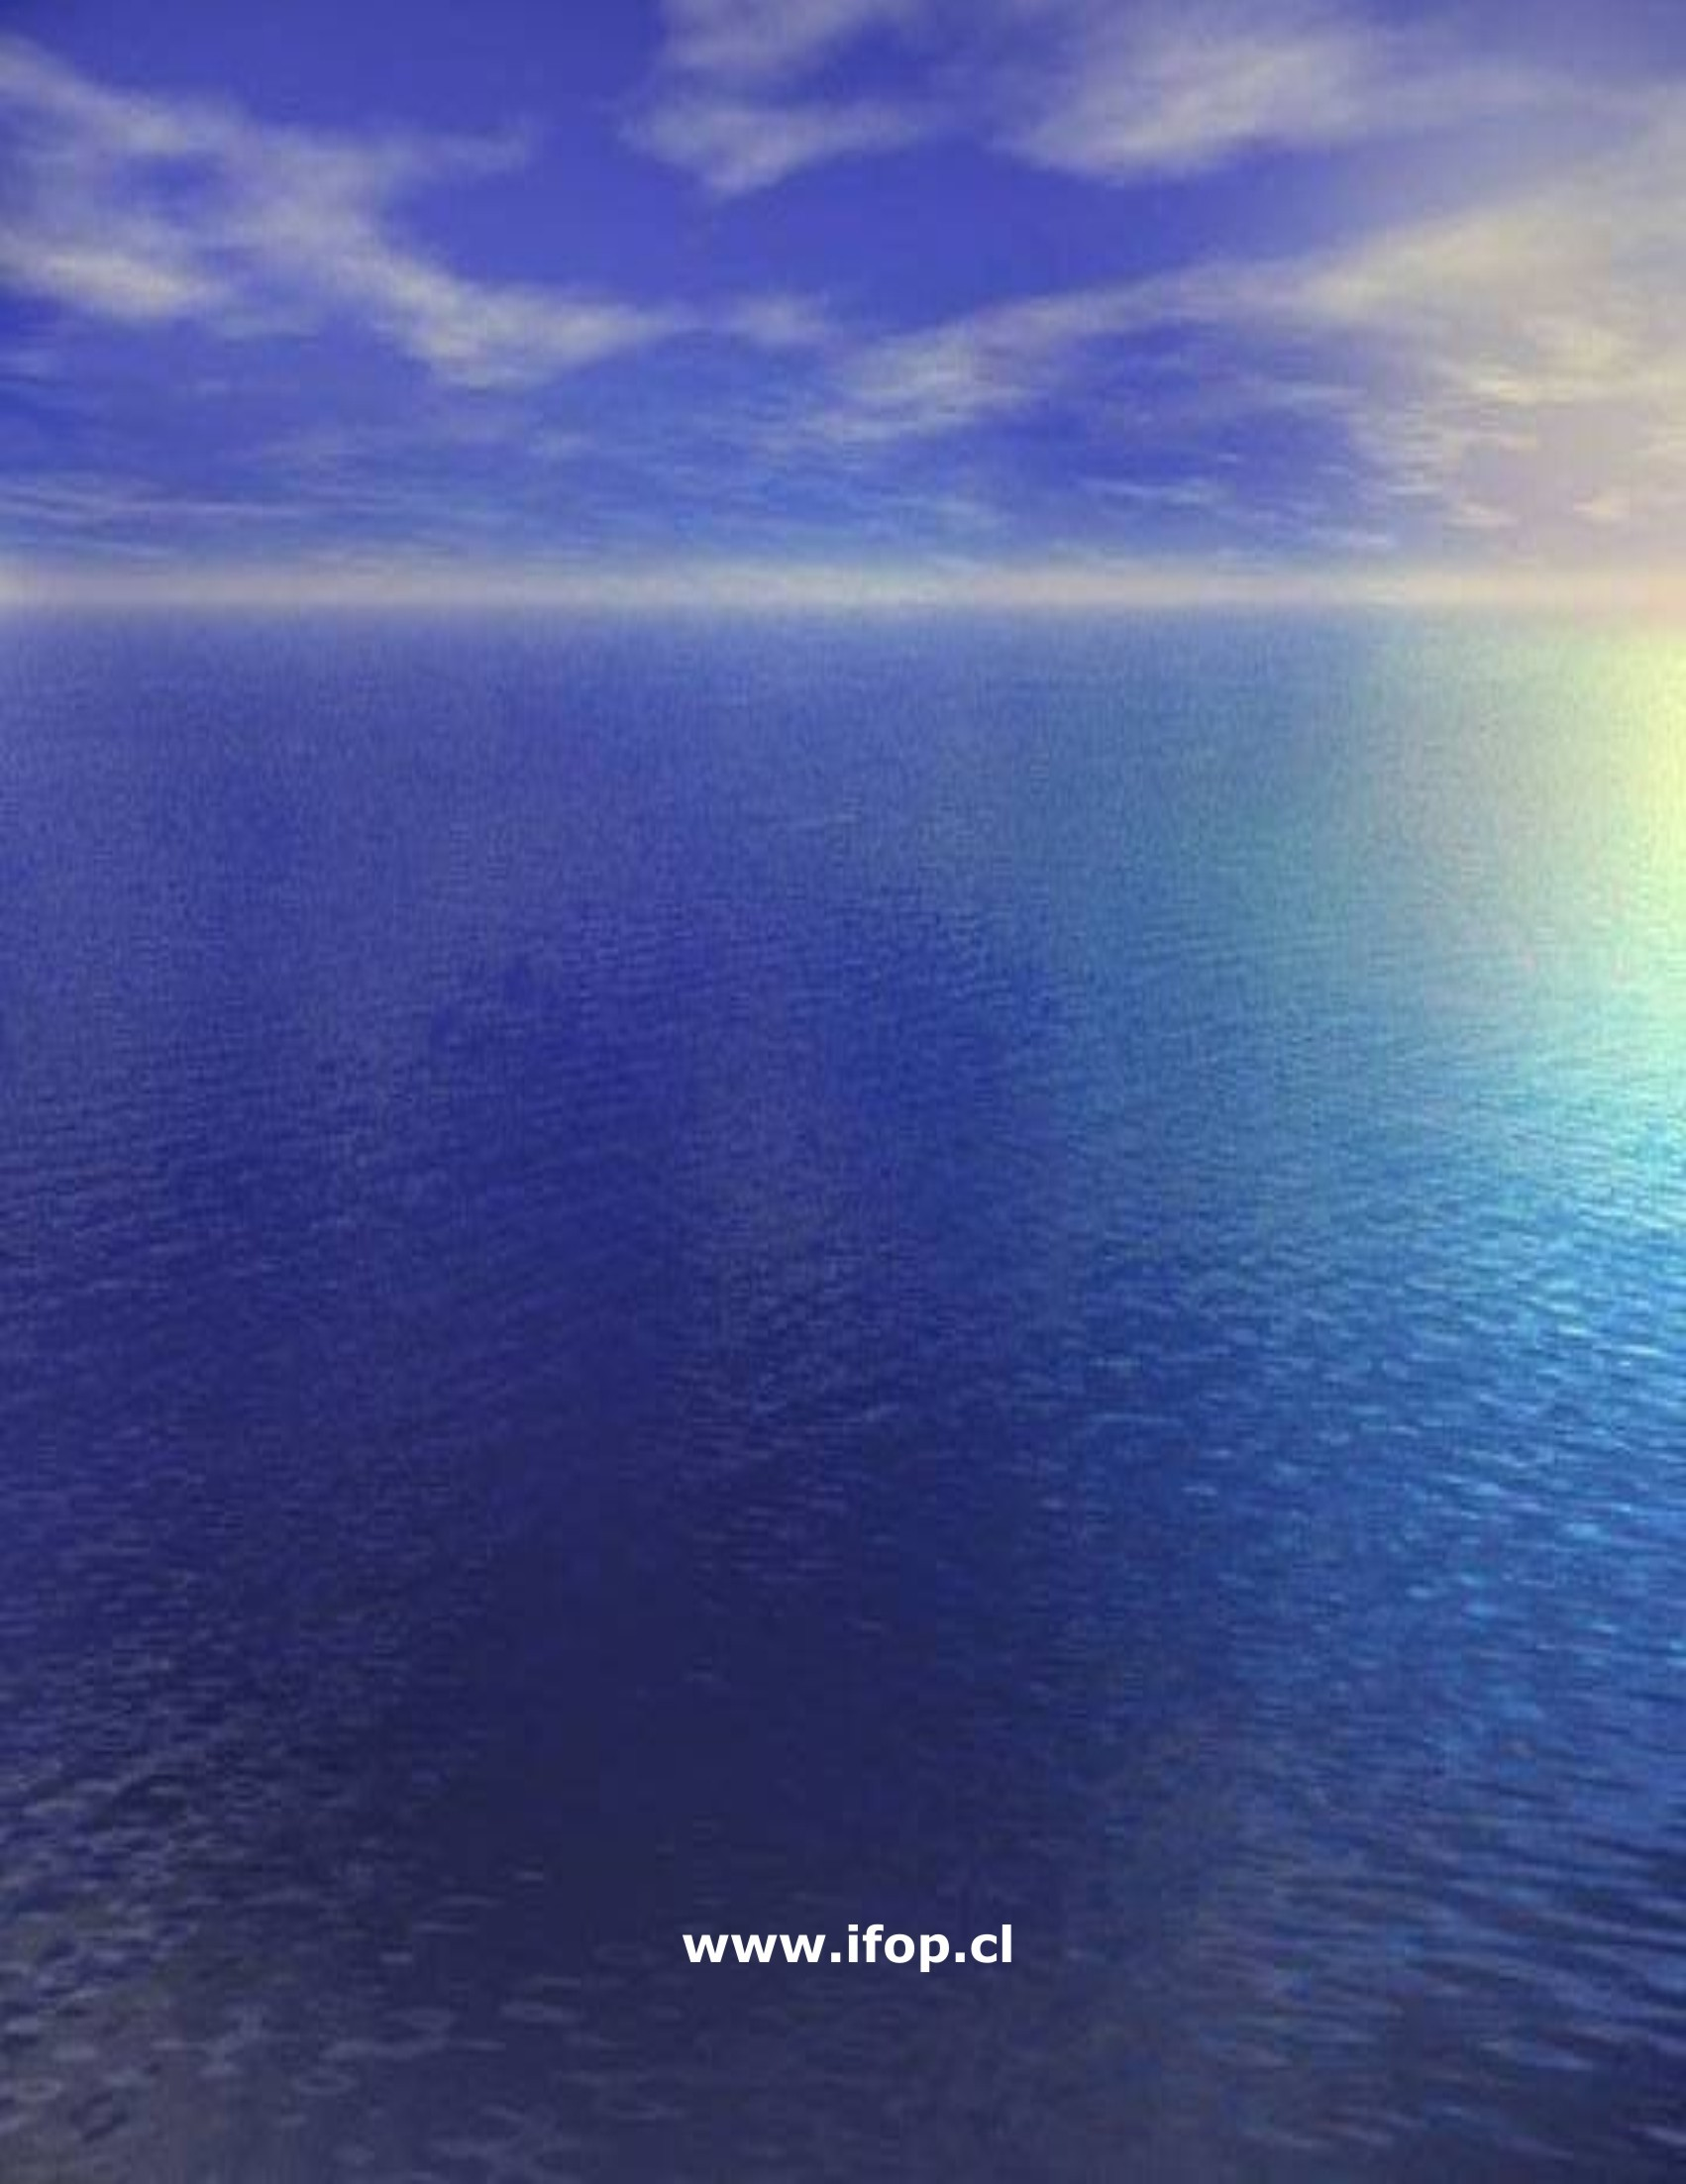
\includegraphics[scale=1]{Figuras/Portada_Final.jpg}}} % Image background
    \noindent
    \vspace{5mm}
      
\end{titlepage}
\endgroup


\end{document}